\documentclass[8pt]{beamer}
\usepackage{tikz,pgfplots,etoolbox}
\usepackage{tkz-berge}
\usetikzlibrary{arrows,decorations.markings,positioning}
\usepackage[breakable,most]{tcolorbox}
\usepackage{colortbl}
\usepackage[T1]{fontenc}
\usefonttheme{serif}
\setbeamercolor{local structure}{fg=black}
%\input{PreCalcLayout}
\graphicspath{ {../Images/} }

%%%% Graph Theory Vertex Label
\newcommand\extralabel[4][0mm]{\node[label={[label distance=#1]#3:#4}] at (#2){};}
% looks like \extralabel[distance(optional)]{node name}{angle}{label text}

% middle arrows on graphs
\tikzset{->-/.style={
 decoration={
   markings,
   mark=at position #1 with {\arrow{>}}
   },
   postaction={decorate}
  },
  ->-/.default=0.5 % set default value for arrow position
}
%\newcommand{\tikzmark}[2]{\tikz[overlay, remember picture] \node[inner sep=5pt, outer sep=5pt, anchor=base] (#1) {#2};}

\newcommand{\extitle}[1]{\frametitle{\fontfamily{fvs}\selectfont \small\color{black!70!blue!80!cyan}\uppercase{\bfseries Example: #1}}}

\def\solblank{\begin{tcolorbox}[colframe=black!50!blue!50!cyan,
colback=white,
bottomrule=0mm,
rightrule=0mm,
sharp corners=all] 
\vspace{6in}
\text{}
\end{tcolorbox}}

\newenvironment{exsol}
{
\begin{tcolorbox}[colframe=black!50!blue!50!cyan,
colback=white,
bottomrule=0mm,
rightrule=0mm,
sharp corners=all] 
%\Large\color{black!70!blue!80!cyan}\scshape #2}\\
}
{ \vspace{6in}
\text{}
\end{tcolorbox}}

\begin{document}

% Section 1.2
\begin{frame}
\extitle{Setting up Percentage Problems}
\begin{enumerate}[(a)]
\item What is 75\% of 690?
\item Forty is what percentage of 150?
\item Eight is 62\% of what?
\end{enumerate}

\solblank
\end{frame}

\begin{frame}
\extitle{Setting up Percentage Problems}
\begin{enumerate}[(a)]
\item What is 75\% of 690?
\end{enumerate}

\solblank
\end{frame}

\begin{frame}
\extitle{Setting up Percentage Problems}
\begin{enumerate}[(a)]
\setcounter{enumi}{1}
\item Forty is what percentage of 150?
\end{enumerate}

\solblank
\end{frame}

\begin{frame}
\extitle{Setting up Percentage Problems}
\begin{enumerate}[(a)]
\setcounter{enumi}{2}
\item Eight is 62\% of what?
\end{enumerate}

\solblank
\end{frame}

\begin{frame}
\extitle{Discount}
For months you have been wanting a 47'' LCD flat screen television, but the price has been too high. The store is having a one-day sale on all televisions in the store. For one day only you can take 25\% off any television. The regular price on the television
you want is \$1099.
\begin{enumerate}[(a)]
\item What is the sale price?
\item What will the final price, including sales tax, be if the sales tax rate is 8\%?
\end{enumerate}

\solblank
\end{frame}

% Section 1.3
\begin{frame}
\extitle{Using the TVM Solver}
\text{}
\vfill
\begin{center}
\parbox{3in}{\Large Use the TVM solver on your calculator to find the present value needed if we want a future value of \$5000 in 6 years, if we can earn 4.3\% interest compounded monthly.}
\end{center}
\vfill
\text{}
\end{frame}

% Section 1.4
\begin{frame}
\extitle{Planning for Retirement}
Kevin is 30 years old, and he is preparing to begin saving for retirement.  He expects to retire at age 67, and for planning purposes, he assumes he'll live to age 95.  Based on cursory research, he expects that his investments can average a return of 7\% annually, and after retirement, he will move his money into more conservative investments returning 5\% annually.  In order to be able to withdraw \$3000 per month after retirement, how much should he plan to save each month?

\solblank
\end{frame}

\begin{frame}
\extitle{Planning for Retirement}
Kevin is 30 years old, and he is preparing to begin saving for retirement.  He expects to retire at age 67, and for planning purposes, he assumes he'll live to age 95.  Based on cursory research, he expects that his investments can average a return of 7\% annually, and after retirement, he will move his money into more conservative investments returning 5\% annually.  In order to be able to withdraw \$3000 per month after retirement, how much should he plan to save each month?

\solblank
\end{frame}

\begin{frame}
\extitle{TVM Solver: Savings Annuity}
\text{}
\vfill
\begin{center}
\parbox{3in}{\Large If you deposit \$250 each month into an IRA earning 7\% interest, how much will you have in the account after 35 years?  Use the TVM Solver on your graphing calculator.}
\end{center}
\vfill
\text{}
\end{frame}

\begin{frame}
\extitle{TVM Solver: Payout Annuity}
\text{}
\vfill
\begin{center}
\parbox{3in}{\Large You expect to have \$500,000 in your IRA when you retire, and you want to be able to take monthly withdrawals for a total of 30 years.  If your account earns 8\% interest, how much will you be able to withdraw each month?  Use the TVM Solver on your graphing calculator.}
\end{center}
\vfill
\text{}
\end{frame}

% Section 1.5
\begin{frame}
\extitle{Buying a Condo}
The price of a condominium is \$180,000, and your bank offers a 30-year fixed mortgage at 4\% interest.  You have \$32,000 available right now.
\begin{enumerate}[(a)]
\item Your banker tells you to expect \$5000 in closing costs.  What percentage down payment can you afford?  Will you need mortgage insurance?
\end{enumerate}

\solblank
\end{frame}

\begin{frame}
\extitle{Buying a Condo}
The price of a condominium is \$180,000, and your bank offers a 30-year fixed mortgage at 4\% interest.  You have \$32,000 available right now.
\begin{enumerate}[(a)]
\item Down payment: 15\% (yes, you need mortgage insurance)
\item What will the principal be on the mortgage?
\end{enumerate}

\solblank
\end{frame}

\begin{frame}
\extitle{Buying a Condo}
The price of a condominium is \$180,000, and your bank offers a 30-year fixed mortgage at 4\% interest.  You have \$32,000 available right now.
\begin{enumerate}[(a)]
\item Down payment: 15\% (yes, you need mortgage insurance)
\item Principal: \$153,000
\item What will your monthly P\&I payment be?
\end{enumerate}

\solblank
\end{frame}

\begin{frame}
\extitle{Buying a Condo}
The price of a condominium is \$180,000, and your bank offers a 30-year fixed mortgage at 4\% interest.  You have \$32,000 available right now.
\begin{enumerate}[(a)]
\item Down payment: 15\% (yes, you need mortgage insurance)
\item Principal: \$153,000
\item Monthly P\&I payment: \$730.45
\item In addition to principal and interest, your monthly payment will need to account for property taxes, homeowners insurance, and mortgage insurance, if necessary (find out in part (a)):
\begin{center}
\begin{tabular}{l r}
\textbf{Property Taxes:} & 1.5\% of the home value per year\\
\textbf{Homeowners Insurance:} & \$900 per year\\
\textbf{Mortgage Insurance:} & \$40 per month
\end{tabular}
\end{center}
What will your total monthly payment amount be?
\end{enumerate}

\solblank
\end{frame}

\begin{frame}
\extitle{Buying a Condo}
The price of a condominium is \$180,000, and your bank offers a 30-year fixed mortgage at 4\% interest.  You have \$32,000 available right now.
\begin{enumerate}[(a)]
\item Down payment: 15\% (yes, you need mortgage insurance)
\item Principal: \$153,000
\item Monthly P\&I payment: \$730.45
\item Total monthly payment: \$1070.45
\item How much will you pay in total over 30 years in principal and interest?
\end{enumerate}

\solblank
\end{frame}

\begin{frame}
\extitle{Buying a Condo}
The price of a condominium is \$180,000, and your bank offers a 30-year fixed mortgage at 4\% interest.  You have \$32,000 available right now.
\begin{enumerate}[(a)]
\item Down payment: 15\% (yes, you need mortgage insurance)
\item Principal: \$153,000
\item Monthly P\&I payment: \$730.45
\item Total monthly payment: \$1070.45
\item Total principal and interest: \$262,962
\item How much interest will you pay in total?
\end{enumerate}

\solblank
\end{frame}

\begin{frame}
\extitle{Buying a Condo}
The price of a condominium is \$180,000, and your bank offers a 30-year fixed mortgage at 4\% interest.  You have \$32,000 available right now.
\begin{enumerate}[(a)]
\item Down payment: 15\% (yes, you need mortgage insurance)
\item Principal: \$153,000
\item Monthly P\&I payment: \$730.45
\item Total monthly payment: \$1070.45
\item Total principal and interest: \$262,962
\item Total interest: \$109,962
\end{enumerate}
\end{frame}

\begin{frame}
\extitle{Changing the Interest Rate}
Compare a 30-year fixed-rate loan at 4\% for \$200,000 to the same loan at 3.5\% by finding the total amount paid in interest for both versions.

\solblank
\end{frame}

\begin{frame}
\extitle{Changing the Loan Amount}
Compare a 30-year fixed-rate loan at 4\% for \$200,000 to the same loan for \$180,000 by finding the total amount paid in interest for both versions.

\solblank
\end{frame}

\begin{frame}
\extitle{Changing the Length of the Loan}
Compare a 30-year fixed-rate loan at 4\% for \$200,000 to the same loan for 20 years and for 15 years by finding the total amount paid in interest for all three versions.

\solblank
\end{frame}

% Section 1.6
\begin{frame}
\extitle{Income Tax}
Using the tax table for 2020, how much would a married taxpayer who files separately from their spouse owe on a taxable income of \$98,400?

\begin{exsol}
{\footnotesize\begin{tabular}{| p{0.5in} | p{1in} |}
\hline
\cellcolor{brown!25}Tax Rate & \cellcolor{brown!25}\parbox{1.3in}{\text{}\\ Single or\\ Married Filing\\ Separately\\ \text{}}\\
\hline
\cellcolor{brown!25}10\% & up to \$9,875\\
\hline
\cellcolor{brown!25}12\% & \$9,875 to \$40,125\\
\hline
\cellcolor{brown!25}22\% & \$40,125 to \$85,525\\
\hline
\cellcolor{brown!25}24\% & \$85,525 to \$163,300\\
\hline
\cellcolor{brown!25}32\% & \$163,300 to \$207,350\\
\hline
\cellcolor{brown!25}35\% & \$207,350 to \$518,400\\
\hline
\cellcolor{brown!25}37\% & more than \$518,400\\
\hline
\cellcolor{brown!25}\parbox{0.9in}{\text{}\\ Standard\\ Deduction\\ \text{}} & \$12,400\\
\hline
\end{tabular}}
\end{exsol}
\end{frame}

\begin{frame}
\extitle{Tax Calculation}
Use the 2020 tax table in the textbook to calculate the final tax owed by a single taxpayer whose details are given below.
\begin{center}
\begin{tabular}{r l}
Gross income: & \$65,000\\
Deductions: & \$3000: charitable donations\\
& \$6000: contribution to traditional IRA\\
& \$1500: education expenses\\
& \$300: cost of tax preparation\\
Tax credit: & \$500: energy-efficient appliances
\end{tabular}
\end{center}

\begin{exsol}
{\footnotesize\begin{tabular}{| p{0.5in} | p{1in} |}
\hline
\cellcolor{brown!25}Tax Rate & \cellcolor{brown!25}\parbox{1.3in}{\text{}\\ Single or\\ Married Filing\\ Separately\\ \text{}}\\
\hline
\cellcolor{brown!25}10\% & up to \$9,875\\
\hline
\cellcolor{brown!25}12\% & \$9,875 to \$40,125\\
\hline
\cellcolor{brown!25}22\% & \$40,125 to \$85,525\\
\hline
\cellcolor{brown!25}24\% & \$85,525 to \$163,300\\
\hline
\cellcolor{brown!25}32\% & \$163,300 to \$207,350\\
\hline
\cellcolor{brown!25}35\% & \$207,350 to \$518,400\\
\hline
\cellcolor{brown!25}37\% & more than \$518,400\\
\hline
\cellcolor{brown!25}\parbox{0.9in}{\text{}\\ Standard\\ Deduction\\ \text{}} & \$12,400\\
\hline
\end{tabular}}
\end{exsol}
\end{frame}

\begin{frame}
\extitle{Tax Calculation}
Use the 2020 tax table in the textbook to calculate the final tax owed by a single taxpayer whose details are given below.
\begin{center}
\begin{tabular}{r l}
Gross income: & \$65,000\\
Deductions: & \$3000: charitable donations\\
& \$6000: contribution to traditional IRA\\
& \$1500: education expenses\\
& \$300: cost of tax preparation\\
Tax credit: & \$500: energy-efficient appliances
\end{tabular}
\end{center}

\begin{exsol}
{\footnotesize\begin{tabular}{| p{0.5in} | p{1in} |}
\hline
\cellcolor{brown!25}Tax Rate & \cellcolor{brown!25}\parbox{1.3in}{\text{}\\ Single or\\ Married Filing\\ Separately\\ \text{}}\\
\hline
\cellcolor{brown!25}10\% & up to \$9,875\\
\hline
\cellcolor{brown!25}12\% & \$9,875 to \$40,125\\
\hline
\cellcolor{brown!25}22\% & \$40,125 to \$85,525\\
\hline
\cellcolor{brown!25}24\% & \$85,525 to \$163,300\\
\hline
\cellcolor{brown!25}32\% & \$163,300 to \$207,350\\
\hline
\cellcolor{brown!25}35\% & \$207,350 to \$518,400\\
\hline
\cellcolor{brown!25}37\% & more than \$518,400\\
\hline
\cellcolor{brown!25}\parbox{0.9in}{\text{}\\ Standard\\ Deduction\\ \text{}} & \$12,400\\
\hline
\end{tabular}}
\end{exsol}
\end{frame}

% Section 2.2
\begin{frame}
\extitle{Plotting Points on a Calculator}
According to the U.S. Census Bureau, the number of Americans over the age of 100 is increasing.  The Census Bureau reported the following data, where the number of people is measured in the thousands:
\begin{center}
\begin{tabular}{c c}
\textbf{Year} & \textbf{Number}\\
& \textbf{(thousands)}\\
\hline
& \\
1994 & 50\\
1996 & 56\\
1998 & 65\\
2000 & 75\\
2002 & 94\\
2004 & 110
\end{tabular}
\end{center}

Graph this data using a graphing calculator.
\end{frame}

\begin{frame}
\extitle{Fitting a Quadratic Model on a Calculator}
According to the U.S. Census Bureau, the number of Americans over the age of 100 is increasing.  The Census Bureau reported the following data, where the number of people is measured in the thousands:
\begin{center}
\begin{tabular}{c c}
\textbf{Year} & \textbf{Number}\\
& \textbf{(thousands)}\\
\hline
& \\
1994 & 50\\
1996 & 56\\
1998 & 65\\
2000 & 75\\
2002 & 94\\
2004 & 110
\end{tabular}
\end{center}
Use a graphing calculator to find a quadratic model that can be used to predict how many Americans will be over the age of 100 in a given year.
\end{frame}

\begin{frame}
\extitle{Making Predictions with a Quadratic Model}
A study designed to track the gas mileage of a car based on its speed found the following results.
\begin{center}
\begin{tabular}{c c}
\textbf{Speed (mph)} & \textbf{Mileage (mpg)}\\
\hline
& \\
15 & 22.3\\
20 & 25.5\\
25 & 27.5\\
30 & 29.0\\
35 & 28.8\\
40 & 30.0\\
45 & 29.9\\
50 & 30.2\\
55 & 30.4\\
60 & 28.8\\
65 & 27.4\\
70 & 25.3\\
75 & 23.3
\end{tabular}
\end{center}

\begin{enumerate}[(a)]
\item Use a graphing calculator to plot the data.
\item Find a quadratic model that best fits the data.
\item Based on this model, what gas mileage should be expected at 62 miles per hour?  At 90 miles per hour?  Which of these predictions is likely to be more reliable?
\item Based on the model, what speeds are likely to produce a mileage of 28 miles per gallon?
\end{enumerate}
\vspace{1in}
\text{}
\end{frame}

\begin{frame}
\extitle{Making Predictions with a Quadratic Model}
\begin{enumerate}[(a)]
\item Use a graphing calculator to plot the data. $\checkmark$
\item Quadratic model: $P_t = -0.008t^2 + 0.746t + 13.469$
\item Based on this model, what gas mileage should be expected at 62 miles per hour?  At 90 miles per hour?  Which of these predictions is likely to be more reliable?
\item Based on the model, what speeds are likely to produce a mileage of 28 miles per gallon?
\end{enumerate}

\solblank
\end{frame}

% Section 2.3
\begin{frame}
\extitle{Solving an Exponential Model for Time}
\begin{center}
\parbox{3in}{\Large In a previous example, we modeled the population growth of Frederick County from 2013 onward using the following equation:
\[P_t = 241,409(1+0.008)^t\]
Use a graphing calculator to find when this model predicts that the population will reach 400,000 people.}
\end{center}
\end{frame}

\begin{frame}
\extitle{Exponential Regression}
Use a graphing calculator to build an exponential population model for the U.S. using data from 2005 to 2019, shown in the table below.
\begin{center}
\begin{tabular}{c c}
\textbf{Year} & \textbf{Population (in millions)}\\
\hline
& \\
2005 & 295.5\\
2006 & 298.4\\
2007 & 301.2\\
2008 & 304.1\\
2009 & 306.8\\
2010 & 309.3\\
2011 & 311.6\\
2012 & 313.9\\
2013 & 316.1\\
2014 & 318.4\\
2015 & 320.7\\
2016 & 323.1\\
2017 & 325.1\\
2018 & 327.2\\
2019 & 328.2
\end{tabular}
\end{center}
\vspace{1.5in}
\text{}
\end{frame}

% Section 2.4
\begin{frame}
\extitle{Logistic Regression}
Use a graphing calculator to build a logistic population model for New York City using the population data below.
\begin{center}
\begin{tabular}{c c}
\textbf{Year} & \textbf{Population (millions)}\\
\hline
& \\
1900 & 3.44\\
1910 & 4.77\\
1920 & 5.62\\ 
1930 & 6.93\\
1940 & 7.45\\
1950 & 7.89\\
1960 & 7.78\\
1970 & 7.89\\
\end{tabular}
\end{center}
\vspace{1.5in}
\text{}
\end{frame}

% Section 3.1
\begin{frame}
\extitle{Representative Samples}
Decide whether each of the following sampling methods is likely to produce a representative sample.

\begin{enumerate}[(a)]
\item To find the average annual income of all adults in the United States, sample representatives in the US Congress.
\vfill

\item To find out the most popular cereal among children under the age of 10, stand outside a large supermarket one day and poll every twentieth child under the age of 10 who enters the supermarket.
\vfill
\text{}
\end{enumerate}
\end{frame}

\begin{frame}
\extitle{Sampling Methods}
Determine the type of sampling used in each of the following scenarios.

\begin{enumerate}[(a)]
\item A soccer coach selects six players from a group of boys aged eight to ten, seven players from a group of boys aged 11 to 12, and three players from a group of boys aged 13 to 14 to form a recreational soccer team.
\vfill

\item A pollster interviews all human resource personnel in five different high tech companies.
\vfill

\item A high school educational counselor interviews 50 female teachers and 50 male teachers.
\vfill
\text{}
\end{enumerate}
\end{frame}

\begin{frame}
\extitle{Sampling Methods}
Determine the type of sampling used in each of the following scenarios.

\begin{enumerate}[(a)]
\setcounter{enumi}{3}
\item A medical researcher interviews every third cancer patient from a list of cancer patients at a local hospital.
\vfill

\item A high school counselor uses a computer to generate 50 random numbers and then picks students whose names correspond to the numbers.
\vfill

\item A student interviews classmates in his algebra class to determine how many pairs of jeans a student at his school owns, on the average.
\vfill
\text{}
\end{enumerate}
\end{frame}

\begin{frame}
\extitle{Quiz Score Samples}
Use the random number generator on your calculator to generate a simple random sample from the data below.  Find the average score for this sample.\\

This table displays six sets of quiz scores (out of 10 points) for an elementary statistics class.
\begin{center}
\begin{tabular}{l l l l l l}
A & B & C & D & E & F\\
\hline
& & & & & \\
5 & 7 & 10 & 9 & 8 & 3\\
10 & 5 & 9 & 8 & 7 & 6\\
9 & 10 & 8 & 6 & 7 & 9\\
9 & 10 & 10 & 9 & 8 & 9\\
7 & 8 & 9 & 5 & 7 & 4\\
9 & 9 & 9 & 10 & 8 & 7\\
7 & 7 & 10 & 9 & 8 & 8\\
8 & 8 & 9 & 10 & 8 & 8\\
9 & 7 & 8 & 7 & 7 & 8\\
8 & 8 & 10 & 9 & 8 & 7\\
\end{tabular}
\end{center}

\solblank
\end{frame}

% Section 3.2
\begin{frame}
\extitle{Dot Plot}
Draw a dot plot to summarize the following data, the ages of 30 randomly chosen NBA players:
\[22, 28, 20, 24, 26, 21, 27, 28, 31, 29, 24, 22, 21, 25, 22,\]
\[25, 30, 29, 20, 22, 36, 24, 23, 36, 24, 29, 21, 21, 26, 23\]

\solblank
\end{frame}

\begin{frame}
\extitle{Categorical Frequency Distribution}
Create a frequency table for the players' positions from the NBA dataset (shown below), including a relative frequency column.
\begin{center}
\begin{tabular}{c c c c c c c c c c}
PF & SF & SG & PG & SG & PF & C & SG & SF & SF\\
PF & PF & SF & SF & PF & SF & SG & PG & PG & C\\
PG & SF & SG & SG & C & SG & C & SG & C & SG
\end{tabular}
\end{center}

\solblank
\end{frame}

\begin{frame}
\extitle{Grouped Frequency Distribution}
Build a grouped frequency table for points per game for the NBA players dataset (shown below), using a class width of 5.
\begin{center}
\begin{tabular}{c c c c c c c c c c}
23.4 & 14.5 & 14.3 & 16.4 & 4.9 & 5.1 & 17.7 & 10.3 & 8.3 & 20.9\\
5.8 & 12.2 & 1.4 & 5.8 & 13.5 & 21.8 & 21.5 & 8.6 & 2.0 & 6.9\\
7.7 & 3.0 & 9.0 & 15.3 & 6.4 & 4.3 & 9.0 & 6.8 & 17.8 & 24.0
\end{tabular}
\end{center}

\solblank
\end{frame}

\begin{frame}
\extitle{Histogram}
Build a histogram for points per game in the NBA dataset (shown below), using grouped classes with a class width of 5.
\begin{center}
\begin{tabular}{c c c c c c c c c c}
23.4 & 14.5 & 14.3 & 16.4 & 4.9 & 5.1 & 17.7 & 10.3 & 8.3 & 20.9\\
5.8 & 12.2 & 1.4 & 5.8 & 13.5 & 21.8 & 21.5 & 8.6 & 2.0 & 6.9\\
7.7 & 3.0 & 9.0 & 15.3 & 6.4 & 4.3 & 9.0 & 6.8 & 17.8 & 24.0
\end{tabular}
\end{center}

\solblank
\end{frame}

\begin{frame}
\extitle{Bar Chart}
Build a bar chart for the players' positions in the NBA dataset (shown below).
\begin{center}
\begin{tabular}{c c c c c c c c c c}
PF & SF & SG & PG & SG & PF & C & SG & SF & SF\\
PF & PF & SF & SF & PF & SF & SG & PG & PG & C\\
PG & SF & SG & SG & C & SG & C & SG & C & SG
\end{tabular}
\end{center}

\solblank
\end{frame}

\begin{frame}
\extitle{Stem and Leaf Plot}
Suppose you gathered data on how long it took you to get ready in the morning.  For 40 days, you measured the amount of time between when your alarm went off and when you left the house.  The results are below, rounded to the nearest minute:
\begin{center}
\begin{tabular}{c c c c c c c c c c}
35 & 28 & 25 & 23 & 23 & 32 & 29 & 19 & 21 & 13\\
24 & 26 & 25 & 31 & 30 & 20 & 25 & 29 & 37 & 26\\
32 & 36 & 18 & 17 & 15 & 24 & 21 & 16 & 19 & 30\\
38 & 27 & 22 & 24 & 28 & 17 & 31 & 32 & 21 & 28\\
\end{tabular}
\end{center}
Build a stem-and-leaf plot for this data.

\solblank
\end{frame}

\begin{frame}
\extitle{Scatterplot: TV Price}
{\footnotesize The following table shows, for a sample of Samsung LCD TVs, their size and their price.  Construct a scatterplot for this data.
\begin{center}
\begin{tabular}{c c | c c | c c}
Size (in.) & Price (\$) & Size (in.) & Price (\$) & Size (in.) & Price (\$)\\
\hline
\\
43 & 500 & 60 & 1200 & 60 & 2800\\
55 & 900 & 45 & 1600 & 22 & 300\\
51 & 900 & 19 & 200 & 60 & 1100\\
32 & 400 & 55 & 2200 & 40 & 600\\
51 & 1200 & 60 & 1700 & 46 & 1600\\
37 & 500 & 55 & 2000 & 40 & 900
\end{tabular}
\end{center}}

\solblank
\end{frame}

\begin{frame}
\extitle{Median NBA Salary}
Find the median of the salaries listed in the NBA dataset (shown below).
\begin{center}
\begin{tabular}{c c c c c c c c c c}
\$155,647 & 
\$384,541 & 
\$898,310 & 
\$898,310 & 
\$898,310\\
\$898,310 & 
\$898,310 & 
\$1,618,420 & 
\$1,620,564 & 
\$1,845,301\\ 
\$2,338,847 & 
\$2,578,800 & 
\$3,625,760 & 
\$3,831,840 & 
\$4,469,160\\
\$4,767,000 & 
\$4,767,000 & 
\$5,500,000 & 
\$7,059,480 & 
\$7,333,333\\
\$7,666,667 & 
\$7,830,000 & 
\$7,839,960 & 
\$8,113,930 & 
\$13,125,000\\
\$13,486,300 & 
\$27,093,019 & 
\$27,504,630 & 
\$30,560,700 & 
\$30,603,448
\end{tabular}
\end{center}

\solblank
\end{frame}

\begin{frame}
\extitle{Weighted Average}
Find the final score of the student whose grades are listed below, using both the points system and the percentage system for defining weights.
\begin{center}
\begin{tabular}{l l l l}
\textbf{Assignment} & \textbf{Score} & \textbf{Weight} & \textbf{Points}\\
\hline
& \\
Test 1 & 85\% & 20\% & 200\\
Test 2 & 92\% & 20\% & 200\\
Test 3 & 87\% & 20\% & 200\\
Homework & 95\% & 15\% & 150\\
Project & 92\% & 10\% & 100\\
Final Exam & 91\% & 15\% & 150
\end{tabular}
\end{center}

\solblank
\end{frame}

\begin{frame}
\extitle{Mode}
Find the mode of the dataset summarized below, the ages of players in the NBA dataset.
\begin{center}
\begin{tabular}{c c}
\textbf{Age} & \textbf{Frequency}\\
\hline
& \\
20 & 2\\
21 & 4\\
22 & 4\\
23 & 2\\
24 & 4\\
25 & 2\\
26 & 2\\
27 & 1\\
28 & 2\\
29 & 3\\
30 & 1\\
31 & 1\\
36 & 2
\end{tabular}
\end{center}
\end{frame}

\begin{frame}
\extitle{Range of NBA Players' Heights}
Find the range of heights for the players listed in the NBA dataset (shown below).
\begin{center}
\begin{tabular}{c c c c c c}
2.03 m & 1.98 m & 1.98 m & 2.08 m & 1.93 m & 2.08 m\\
2.08 m & 1.85 m & 1.98 m & 2.01 m & 2.08 m & 2.01 m\\
2.03 m & 1.98 m & 2.03 m & 2.01 m & 2.03 m & 1.91 m\\
1.93 m & 2.11 m & 1.78 m & 2.06 m & 2.03 m & 1.91 m\\
2.06 m & 1.93 m & 2.06 m & 1.91 m & 2.13 m & 1.85 m
\end{tabular}
\end{center}

\solblank
\end{frame}

% Section 3.4
\begin{frame}
\extitle{Linear Regression with House Prices}
Construct the least-squares regression line for the house price data given below, knowing that $r=0.9$.
\begin{center}
\begin{tabular}{c c}
\textbf{Size (sq. ft.)} & \textbf{Selling Price (\$1000s)}\\
\hline
& \\
2521 & 400\\
2555 & 426\\
2735 & 428\\
2846 & 435\\
3028 & 469\\
3049 & 475\\
3198 & 488\\
3198 & 455\\
\end{tabular}
\end{center}
\end{frame}

\begin{frame}
\extitle{Linear Regression with House Prices}
(continued)\\
Construct the least-squares regression line for the house price data with the statistics below, knowing that $r=0.9$.
\[\overline{x} = 2891, \overline{y} = 447\]
\[s_x = 269.5, s_y = 29.7\]

\solblank
\end{frame}

\begin{frame}
\extitle{Regression Line}
A random sample of 11 statistics students produced the following data, where $x$ is the third exam score out of 80, and $y$ is the final exam score out of 200.
\begin{center}
\begin{tabular}{c c}
$x$ & $y$\\
\hline
\\
65 & 175\\
67 & 133\\
71 & 185\\
71 & 163\\
66 & 126\\
75 & 198\\
67 & 153\\
70 & 163\\
71 & 159\\
69 & 151\\
69 & 159
\end{tabular}
\end{center}

Use a graphing calculator to find the equation of the least-squares regression line that can be used to predict a student's performance on the final exam based on their third test score.
\end{frame}

\begin{frame}
\extitle{Predicting House Values}
Using a sample of houses on the market, we found the following regression equation to predict the price $y$ based on the square footage $x$:
\[\hat{y} = 0.099x + 160.8\]
Use this equation to predict the price of homes with the following square footage values:
\begin{enumerate}[(a)]
\item 2700 square feet
\item 4500 square feet
\end{enumerate}
Which prediction do you expect to be more reliable?

\solblank
\end{frame}

\begin{frame}
\extitle{Linear Regression with NFL Quarterbacks}
The following table lists the heights (in inches) and weights (in pounds) of 10 NFL quarterbacks in the 2019 season.
{\footnotesize\begin{center}
\begin{tabular}{l c c}
\textbf{Name} & \textbf{Height} & \textbf{Weight}\\
\hline
& & \\
Lamar Jackson & 75 & 200\\
Patrick Mahomes & 74 & 225\\
Dak Prescott & 74 & 226\\
Kyler Murray & 70 & 207\\
Russell Wilson & 71 & 206\\
Deshaun Watson & 74 & 221\\
Matt Ryan & 76 & 220\\
Josh Allen & 77 & 233\\
Drew Brees & 72 & 209\\
Aaron Rodgers & 74 & 225\\
\end{tabular}
\end{center}}
\begin{enumerate}[(a)]
\item Calculate the correlation coefficient for this data.
\end{enumerate}

\solblank
\end{frame}

\begin{frame}
\extitle{Linear Regression with NFL Quarterbacks}
The following table lists the heights (in inches) and weights (in pounds) of 10 NFL quarterbacks in the 2019 season.
{\footnotesize\begin{center}
\begin{tabular}{l c c}
\textbf{Name} & \textbf{Height} & \textbf{Weight}\\
\hline
& & \\
Lamar Jackson & 75 & 200\\
Patrick Mahomes & 74 & 225\\
Dak Prescott & 74 & 226\\
Kyler Murray & 70 & 207\\
Russell Wilson & 71 & 206\\
Deshaun Watson & 74 & 221\\
Matt Ryan & 76 & 220\\
Josh Allen & 77 & 233\\
Drew Brees & 72 & 209\\
Aaron Rodgers & 74 & 225\\
\end{tabular}
\end{center}}
\begin{enumerate}[(a)]
\item $r = 0.6$
\item Is there are strong linear relationship?
\end{enumerate}

\solblank
\end{frame}

\begin{frame}
\extitle{Linear Regression with NFL Quarterbacks}
The following table lists the heights (in inches) and weights (in pounds) of 10 NFL quarterbacks in the 2019 season.
{\footnotesize\begin{center}
\begin{tabular}{l c c}
\textbf{Name} & \textbf{Height} & \textbf{Weight}\\
\hline
& & \\
Lamar Jackson & 75 & 200\\
Patrick Mahomes & 74 & 225\\
Dak Prescott & 74 & 226\\
Kyler Murray & 70 & 207\\
Russell Wilson & 71 & 206\\
Deshaun Watson & 74 & 221\\
Matt Ryan & 76 & 220\\
Josh Allen & 77 & 233\\
Drew Brees & 72 & 209\\
Aaron Rodgers & 74 & 225\\
\end{tabular}
\end{center}}
\begin{enumerate}[(a)]
\item $r = 0.6$
\item There is a moderate (positive) linear relationship.
\item Compute the regression line for predicting weight from height.
\end{enumerate}

\solblank
\end{frame}

\begin{frame}
\extitle{Linear Regression with NFL Quarterbacks}
The following table lists the heights (in inches) and weights (in pounds) of 10 NFL quarterbacks in the 2019 season.
{\footnotesize\begin{center}
\begin{tabular}{l c c}
\textbf{Name} & \textbf{Height} & \textbf{Weight}\\
\hline
& & \\
Lamar Jackson & 75 & 200\\
Patrick Mahomes & 74 & 225\\
Dak Prescott & 74 & 226\\
Kyler Murray & 70 & 207\\
Russell Wilson & 71 & 206\\
Deshaun Watson & 74 & 221\\
Matt Ryan & 76 & 220\\
Josh Allen & 77 & 233\\
Drew Brees & 72 & 209\\
Aaron Rodgers & 74 & 225\\
\end{tabular}
\end{center}}
\begin{enumerate}[(a)]
\item $r = 0.6$
\item There is a moderate (positive) linear relationship.
\item Regression line: $\hat{y} = 3.01x - 4.43$
\item Graph the data and the regression equation.
\end{enumerate}
\vspace{3in}
\text{}
\end{frame}

\begin{frame}
\extitle{Linear Regression with NFL Quarterbacks}
The following table lists the heights (in inches) and weights (in pounds) of 10 NFL quarterbacks in the 2019 season.
{\footnotesize\begin{center}
\begin{tabular}{l c c}
\textbf{Name} & \textbf{Height} & \textbf{Weight}\\
\hline
& & \\
Lamar Jackson & 75 & 200\\
Patrick Mahomes & 74 & 225\\
Dak Prescott & 74 & 226\\
Kyler Murray & 70 & 207\\
Russell Wilson & 71 & 206\\
Deshaun Watson & 74 & 221\\
Matt Ryan & 76 & 220\\
Josh Allen & 77 & 233\\
Drew Brees & 72 & 209\\
Aaron Rodgers & 74 & 225\\
\end{tabular}
\end{center}}
\begin{enumerate}[(a)]
\item $r = 0.6$
\item There is a moderate (positive) linear relationship.
\item Regression line: $\hat{y} = 3.01x - 4.43$
\item Graph the data and the regression equation.
\end{enumerate}

\begin{center}
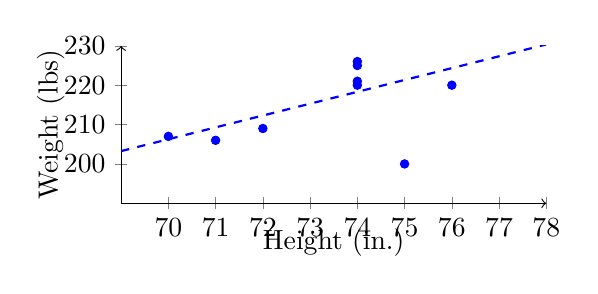
\begin{tikzpicture}
\begin{axis}[
    xmin=69, xmax=78,
    ymin=190, ymax=230,
    axis lines=center,
    axis on top=false,
    domain=0:1,
    x=0.6cm,
    y=0.05cm,
    xtick={69,70,...,78},
    xticklabels={69,70,...,78},
    ytick={190,200,...,230},
    yticklabels={190,200,...,230},
    axis lines=middle,
    axis line style={->},
    x label style={at={(axis description cs:0.5,-0.1)},anchor=north},
    y label style={at={(axis description cs:-0.11,.5)},rotate=90,anchor=south},
    xlabel={Height (in.)},
    ylabel={Weight (lbs)},
    grid=none
    ]
	\addplot [blue,only marks,mark size=1.5] table[row sep=crcr] {
	75 200\\
	74 220\\
	74 226\\
	70 207\\
	71 206\\
	74 221\\
	76 220\\
	77 233\\
	72 209\\
	74 225\\
	};
	\addplot [blue, dashed, thick, domain=69:78, samples=10] {3.01*x-4.43};
\end{axis}
\end{tikzpicture}
\end{center}
\end{frame}

\begin{frame}
\extitle{Linear Regression with NFL Quarterbacks}
The following table lists the heights (in inches) and weights (in pounds) of 10 NFL quarterbacks in the 2019 season.
{\footnotesize\begin{center}
\begin{tabular}{l c c}
\textbf{Name} & \textbf{Height} & \textbf{Weight}\\
\hline
& & \\
Lamar Jackson & 75 & 200\\
Patrick Mahomes & 74 & 225\\
Dak Prescott & 74 & 226\\
Kyler Murray & 70 & 207\\
Russell Wilson & 71 & 206\\
Deshaun Watson & 74 & 221\\
Matt Ryan & 76 & 220\\
Josh Allen & 77 & 233\\
Drew Brees & 72 & 209\\
Aaron Rodgers & 74 & 225\\
\end{tabular}
\end{center}}
\begin{enumerate}[(a)]
\item $r = 0.6$
\item There is a moderate (positive) linear relationship.
\item Regression line: $\hat{y} = 3.01x - 4.43$
\item Graph the data and the regression equation. $\checkmark$
\item Predict the weight of a quarterback who is 73 inches tall.
\end{enumerate}

\solblank
\end{frame}

\begin{frame}
\extitle{Linear Regression with NFL Quarterbacks}
The following table lists the heights (in inches) and weights (in pounds) of 10 NFL quarterbacks in the 2019 season.
{\footnotesize\begin{center}
\begin{tabular}{l c c}
\textbf{Name} & \textbf{Height} & \textbf{Weight}\\
\hline
& & \\
Lamar Jackson & 75 & 200\\
Patrick Mahomes & 74 & 225\\
Dak Prescott & 74 & 226\\
Kyler Murray & 70 & 207\\
Russell Wilson & 71 & 206\\
Deshaun Watson & 74 & 221\\
Matt Ryan & 76 & 220\\
Josh Allen & 77 & 233\\
Drew Brees & 72 & 209\\
Aaron Rodgers & 74 & 225\\
\end{tabular}
\end{center}}
\begin{enumerate}[(a)]
\item $r = 0.6$
\item There is a moderate (positive) linear relationship.
\item Regression line: $\hat{y} = 3.01x - 4.43$
\item Graph the data and the regression equation. $\checkmark$
\item Predict the weight of a quarterback who is 73 inches tall: 215.3 pounds
\item Does Drew Brees weigh more or less than the weight predicted by the regression line, based on his height?
\end{enumerate}

\solblank
\end{frame}

\begin{frame}
\extitle{Linear Regression with NFL Quarterbacks}
\begin{enumerate}[(a)]
\item $\boxed{r = 0.6}$
\item There is a $\boxed{\textrm{moderate}}$ (positive) linear relationship.
\item Regression line: $\boxed{\hat{y} = 3.01x - 4.43}$
\item Graph the data and the regression equation.

\begin{center}
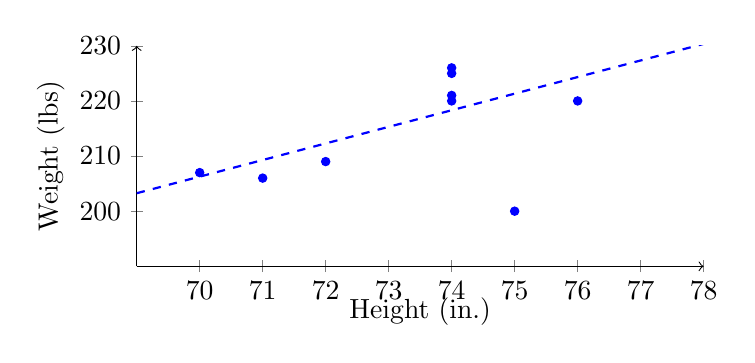
\begin{tikzpicture}
\begin{axis}[
    xmin=69, xmax=78,
    ymin=190, ymax=230,
    axis lines=center,
    axis on top=false,
    domain=0:1,
    x=0.8cm,
    y=0.07cm,
    xtick={69,70,...,78},
    xticklabels={69,70,...,78},
    ytick={190,200,...,230},
    yticklabels={190,200,...,230},
    axis lines=middle,
    axis line style={->},
    x label style={at={(axis description cs:0.5,-0.1)},anchor=north},
    y label style={at={(axis description cs:-0.11,.5)},rotate=90,anchor=south},
    xlabel={Height (in.)},
    ylabel={Weight (lbs)},
    grid=none
    ]
	\addplot [blue,only marks,mark size=1.5] table[row sep=crcr] {
	75 200\\
	74 220\\
	74 226\\
	70 207\\
	71 206\\
	74 221\\
	76 220\\
	77 233\\
	72 209\\
	74 225\\
	};
	\addplot [blue, dashed, thick, domain=69:78, samples=10] {3.01*x-4.43};
\end{axis}
\end{tikzpicture}
\end{center}

\item Predict the weight of a quarterback who is 73 inches tall: $\boxed{\textrm{215.3 pounds}}$
\item Does Drew Brees weigh more or less than the weight predicted by the regression line, based on his height? $\boxed{\textrm{Less}}$
\end{enumerate}
\end{frame}

% Section 3.5
\begin{frame}
\extitle{Sample Size for Poll}
If you want a poll to have a margin of error of 2\% or less, what's the minimum sample size you should use?

\solblank
\end{frame}

% Section 4.3
\begin{frame}
\extitle{Probability with M\&M's}
A bag of M\&M's contains the following breakdown of colors:

\begin{center}
\begin{tabular}{c c c c c c}
\textbf{Red} & \textbf{Yellow} &  \textbf{Brown} & \textbf{Blue} & \textbf{Orange} & \textbf{Green} \\ \hline
& & & & & \\
12 & 18 & 24 &  22 &  13 & 17 \\
\end{tabular}
\end{center}
Suppose you pull two M\&M's out of the bag (without replacing the candy after each pull).\\ \text{}\\

\begin{enumerate}[(a)]
\item Find the probability of drawing two red candies
\end{enumerate}

\solblank
\end{frame}

\begin{frame}
\extitle{Probability with M\&M's}
A bag of M\&M's contains the following breakdown of colors:

\begin{center}
\begin{tabular}{c c c c c c}
\textbf{Red} & \textbf{Yellow} &  \textbf{Brown} & \textbf{Blue} & \textbf{Orange} & \textbf{Green} \\ \hline
& & & & & \\
12 & 18 & 24 &  22 &  13 & 17 \\
\end{tabular}
\end{center}
Suppose you pull two M\&M's out of the bag (without replacing the candy after each pull).\\ \text{}\\

\begin{enumerate}[(a)]
\setcounter{enumi}{1}
\item Find the probability of drawing a blue candy and then a brown candy, in that order
\end{enumerate}

\solblank
\end{frame}

\begin{frame}
\extitle{Probability with M\&M's}
A bag of M\&M's contains the following breakdown of colors:

\begin{center}
\begin{tabular}{c c c c c c}
\textbf{Red} & \textbf{Yellow} &  \textbf{Brown} & \textbf{Blue} & \textbf{Orange} & \textbf{Green} \\ \hline
& & & & & \\
12 & 18 & 24 &  22 &  13 & 17 \\
\end{tabular}
\end{center}
Suppose you pull two M\&M's out of the bag (without replacing the candy after each pull).\\ \text{}\\

\begin{enumerate}[(a)]
\setcounter{enumi}{2}
\item Find the probability of \textbf{not} drawing two green candies
\end{enumerate}

\solblank
\end{frame}

\begin{frame}
\extitle{Probability with M\&M's}
A bag of M\&M's contains the following breakdown of colors:

\begin{center}
\begin{tabular}{c c c c c c}
\textbf{Red} & \textbf{Yellow} &  \textbf{Brown} & \textbf{Blue} & \textbf{Orange} & \textbf{Green} \\ \hline
& & & & & \\
12 & 18 & 24 &  22 &  13 & 17 \\
\end{tabular}
\end{center}
Suppose you pull two M\&M's out of the bag (without replacing the candy after each pull).\\ \text{}\\

\begin{enumerate}[(a)]
\setcounter{enumi}{3}
\item Find the probability of drawing one orange candy and one yellow candy (note that order is not mentioned)
\end{enumerate}

\solblank
\end{frame}

% Section 8.1
\begin{frame}
\extitle{Classifying Graphs}
For each of the following graphs, determine whether it is a simple graph or multigraph, and whether it is directed or undirected.

\begin{center}
\begin{tabular}{c c c c}
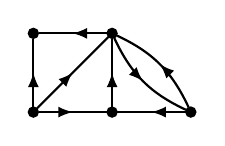
\begin{tikzpicture}
  \GraphInit[vstyle=simple]
  \tikzset{VertexStyle/.append style={scale=0.3}}
  \SetGraphUnit{1}
  \tikzset{EdgeStyle/.style = {->-,>=latex}}
  \Vertex{1}
  \NO(1){2}
  \EA(1){3}
  \NO(3){4}
  \EA(3){5}
  \Edge(1)(2)
  \Edge(1)(3)
  \Edge(1)(4)
  \Edge(4)(2)
  \Edge(3)(4)
  \Edge(5)(3)
  \tikzset{EdgeStyle/.style = {->-,>=latex,bend right=20}}
  \Edge(5)(4)
  \Edge(4)(5)
\end{tikzpicture}
&
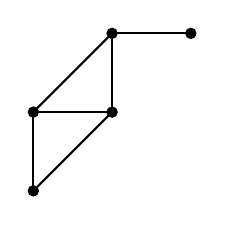
\begin{tikzpicture}
  \GraphInit[vstyle=simple]
  \tikzset{VertexStyle/.append style={scale=0.3}}
  \SetGraphUnit{1}
  \Vertex{1}
  \NO(1){2}
  \EA(2){3}
  \NO(3){4}
  \EA(4){5}
  \Edge(1)(2)
  \Edge(1)(3)
  \Edge(2)(3)
  \Edge(2)(4)
  \Edge(3)(4)
  \Edge(4)(5)
\end{tikzpicture}
&

\begin{tikzpicture}
  \GraphInit[vstyle=simple]
  \tikzset{VertexStyle/.append style={scale=0.3}}
  \SetGraphUnit{1}
  \Vertex{1}
  \NOWE(1){2}
  \SetUpEdge[style={bend right=30}]
  \Edge(1)(2)
  \Edge(2)(1)
  \Loop[dist=1cm,dir=NO,style={-,line width=0.7pt}](2)
\end{tikzpicture}
&
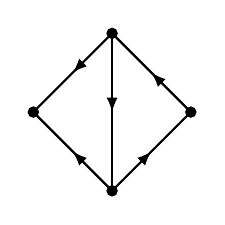
\begin{tikzpicture}
  \GraphInit[vstyle=simple]
  \tikzset{VertexStyle/.append style={scale=0.3}}
  \SetGraphUnit{1}
  \tikzset{EdgeStyle/.style = {->-,>=latex}}
  \Vertex{1}
  \NOWE(1){2}
  \NOEA(1){3}
  \NOEA(2){4}
  \Edge(1)(2)
  \Edge(1)(3)
  \Edge(4)(1)
  \Edge(4)(2)
  \Edge(3)(4)
\end{tikzpicture}\\
& & & \\
(a) & (b) & (c) & (d)
\end{tabular}
\end{center}

\solblank
\end{frame}

\begin{frame}
\extitle{Degrees of Nodes}
Find the degree of each node in the social network graph shown here.
\vspace{0.5in}
\begin{center}
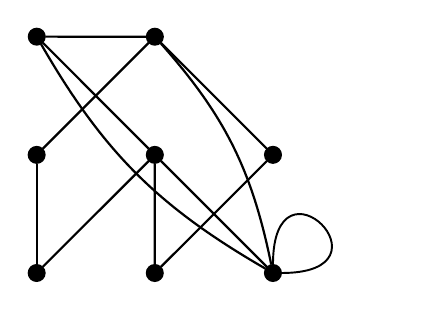
\begin{tikzpicture}[scale=1.5]
  \GraphInit[vstyle=simple]
  \tikzset{VertexStyle/.append style={scale=0.5}}
  \Vertex{Agnes}
  \NO(Agnes){Ellis}
  \EA(Agnes){Marie}
  \NO(Marie){Ivan}
  \NO(Ivan){Tamara}
  \WE(Tamara){Joel}
  \EA(Marie){Musa}
  \EA(Ivan){Kira}
  %\extralabel[1mm]{Agnes}{225}{Agnes}
  %\extralabel[1mm]{Ellis}{180}{Ellis}
  %\extralabel[1mm]{Marie}{-90}{Marie}
  %\extralabel[0.25mm]{Ivan}{80}{Ivan}
  %\extralabel[1mm]{Tamara}{45}{Tamara}
  %\extralabel[1mm]{Joel}{135}{Joel}
  %\extralabel[1mm]{Musa}{-45}{Musa}
  %\extralabel[1mm]{Kira}{0}{Kira}
  \Edge(Agnes)(Ellis)
  \Edge(Agnes)(Ivan)
  \Edge(Ivan)(Marie)
  \Edge(Ivan)(Joel)
  \Edge(Joel)(Tamara)
  \Edge(Tamara)(Kira)
  \Edge(Kira)(Marie)
  \Edge(Ivan)(Musa)
  \Edge(Ellis)(Tamara)
  \SetUpEdge[style={bend right=15}]
  \Edge(Musa)(Tamara)
  \Edge(Joel)(Musa)
  \Loop[dist=1cm,dir=NOEA,style={-,line width=0.7pt}](Musa)
\end{tikzpicture}\\
\vspace{0.5in}
(a)
\end{center}
\end{frame}

\begin{frame}
\extitle{Degrees of Nodes}
Find the degree of each node in the social network graph shown here.
\vspace{0.5in}
\begin{center}
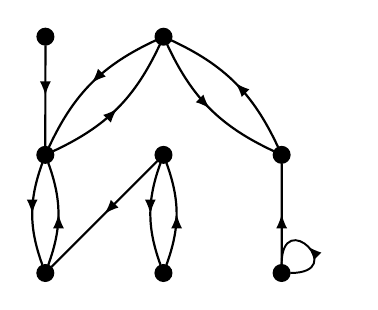
\begin{tikzpicture}[scale=1.5]
  \GraphInit[vstyle=simple]
  \tikzset{VertexStyle/.append style={scale=0.5}}
  \Vertex{Agnes}
  \NO(Agnes){Ellis}
  \EA(Agnes){Marie}
  \NO(Marie){Ivan}
  \NO(Ivan){Tamara}
  \WE(Tamara){Joel}
  \EA(Marie){Musa}
  \EA(Ivan){Kira}
  %\extralabel[1mm]{Agnes}{225}{Agnes}
  %\extralabel[1mm]{Ellis}{180}{Ellis}
  %\extralabel[1mm]{Marie}{-90}{Marie}
  %\extralabel[0.25mm]{Ivan}{92}{Ivan}
  %\extralabel[1mm]{Tamara}{45}{Tamara}
  %\extralabel[1mm]{Joel}{135}{Joel}
  %\extralabel[1mm]{Musa}{-45}{Musa}
  %\extralabel[1mm]{Kira}{0}{Kira}
  
  \tikzset{EdgeStyle/.style = {->-,>=latex}}
  \Edge(Joel)(Ellis)
  \Edge(Ivan)(Agnes)
  \Edge(Musa)(Kira)
  \Loop[dist=0.5cm,dir=NOEA,style={-,line width=0.7pt}](Musa)
  \tikzset{EdgeStyle/.style = {->-,>=latex,bend right=20}}
  \Edge(Agnes)(Ellis)
  \Edge(Ellis)(Agnes)
  \Edge(Marie)(Ivan)
  \Edge(Ivan)(Marie)
  \Edge(Kira)(Tamara)
  \Edge(Tamara)(Kira)
  \Edge(Ellis)(Tamara)
  \Edge(Tamara)(Ellis)
\end{tikzpicture}\\
\vspace{0.5in}
(b)
\end{center}
\end{frame}

% Section 8.2
\begin{frame}
\extitle{Euler Paths in Modern K\"onigsberg}
A modern image of part of Kaliningrad (which was once K\"onigsberg) is shown below, with bridges highlighted.
\begin{center}
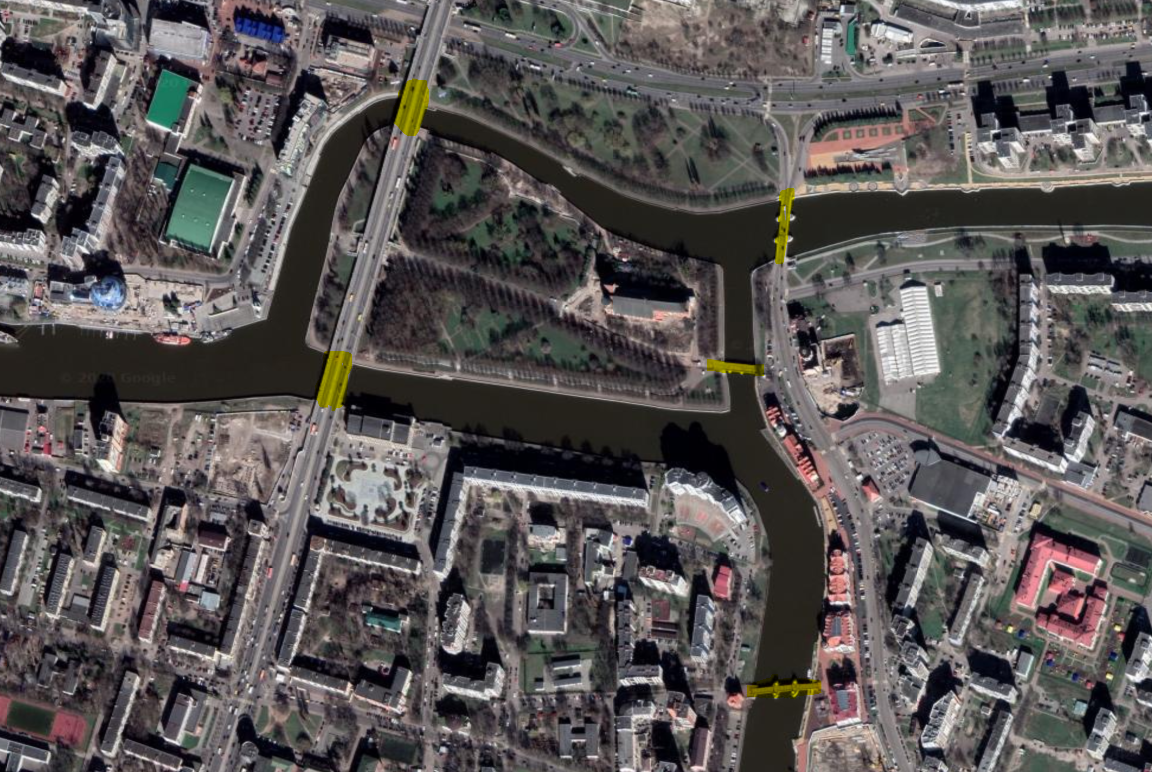
\includegraphics[height=1in]{ModernKonigsberg}
\end{center}
Is there an Euler path and/or circuit through this part of the city?  If so, find one.

\solblank
\end{frame}

\begin{frame}
\extitle{Existence of Euler Paths}
For each of the following graphs, determine if an Euler circuit exists.  If not, determine whether there is an Euler path.
\begin{center}
\begin{tabular}{c c c}
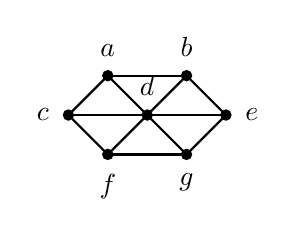
\begin{tikzpicture}
  \GraphInit[vstyle=simple]
  \tikzset{VertexStyle/.append style={scale=0.3}}
  \SetGraphUnit{0.5}
  \Vertex{1}
  \SOWE(1){3}
  \SOEA(1){4}
  \NOEA(4){2}
  \SOEA(2){5}
  \SOEA(3){6}
  \SOEA(4){7}
  
  \extralabel{1}{90}{$a$}
  \extralabel{2}{90}{$b$}
  \extralabel{3}{180}{$c$}
  \extralabel{4}{90}{$d$}
  \extralabel{5}{0}{$e$}
  \extralabel{6}{-90}{$f$}
  \extralabel{7}{-90}{$g$}
  
  \Edge(1)(2)
  \Edge(1)(3)
  \Edge(1)(4)
  \Edge(2)(4)
  \Edge(2)(5)
  \Edge(3)(4)
  \Edge(4)(5)
  \Edge(3)(6)
  \Edge(4)(6)
  \Edge(4)(7)
  \Edge(5)(7)
  \Edge(6)(7)
\end{tikzpicture}
&
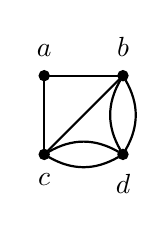
\begin{tikzpicture}
  \GraphInit[vstyle=simple]
  \tikzset{VertexStyle/.append style={scale=0.3}}
  \SetGraphUnit{1}
  \Vertex{a}
  \EA(a){b}
  \SO(a){c}
  \SO(b){d}
  
  \extralabel{a}{90}{$a$}
  \extralabel{b}{90}{$b$}
  \extralabel{c}{-90}{$c$}
  \extralabel{d}{-90}{$d$}
  
  \Edge(a)(b)
  \Edge(a)(c)
  \Edge(b)(c)
  \SetUpEdge[style={bend right=30}]
  \Edge(b)(d)
  \Edge(d)(b)
  \Edge(c)(d)
  \Edge(d)(c)
\end{tikzpicture}
&
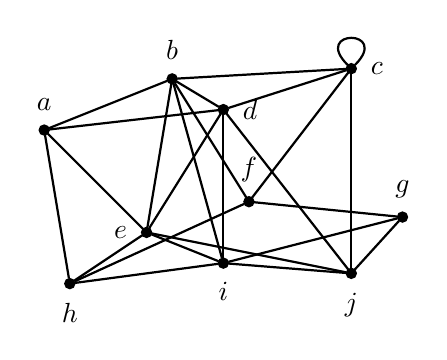
\begin{tikzpicture}[scale=0.65]
  \GraphInit[vstyle=simple]
  \tikzset{VertexStyle/.append style={scale=0.3}}
  \Vertex[x=0,y=0]{a}
  \Vertex[x=2.5,y=1]{b}
  \Vertex[x=6,y=1.2]{c}
  \Vertex[x=3.5,y=0.4]{d}
  \Vertex[x=2,y=-2]{e}
  \Vertex[x=4,y=-1.4]{f}
  \Vertex[x=7,y=-1.7]{g}
  \Vertex[x=0.5,y=-3]{h}
  \Vertex[x=3.5,y=-2.6]{i}
  \Vertex[x=6,y=-2.8]{j}
  
  \extralabel{a}{90}{$a$}
  \extralabel{b}{90}{$b$}
  \extralabel{c}{0}{$c$}
  \extralabel{d}{0}{$d$}
  \extralabel{e}{180}{$e$}
  \extralabel{f}{90}{$f$}
  \extralabel{g}{90}{$g$}
  \extralabel{h}{-90}{$h$}
  \extralabel{i}{-90}{$i$}
  \extralabel{j}{-90}{$j$}
  
  \Edge(a)(b)
  \Edge(a)(d)
  \Edge(a)(e)
  \Edge(a)(h)
  \Edge(b)(c)
  \Edge(b)(d)
  \Edge(b)(e)
  \Edge(b)(f)
  \Edge(b)(i)
  \Edge(c)(d)
  \Edge(c)(f)
  \Edge(c)(j)
  \Edge(d)(e)
  \Edge(d)(j)
  \Edge(d)(i)
  \Edge(e)(h)
  \Edge(e)(i)
  \Edge(e)(j)
  \Edge(f)(g)
  \Edge(f)(h)
  \Edge(g)(i)
  \Edge(g)(j)
  \Edge(h)(i)
  \Edge(i)(j)
  \Loop[dist=1cm,dir=NO,style={-}](c)
\end{tikzpicture}\\
& & \\
(a) & (b) & (c)
\end{tabular}
\end{center}

\solblank
\end{frame}

\begin{frame}
\extitle{Euler Path through House}
The floor plan below shows the first floor of a single-family home.  Is there an Euler circuit/path through the interior of this level, using the highlighted doors (in other words, ignoring external doors and stairs)?
\begin{center}
\includegraphics[width=0.5\textwidth]{Sample_Floorplan}
\end{center}

\solblank
\end{frame}

\begin{frame}
\extitle{Euler Paths in Directed Graphs}
For each of the following graphs, determine if an Euler circuit exists.  If not, determine whether there is an Euler path.
\begin{center}
\begin{tabular}{c c}
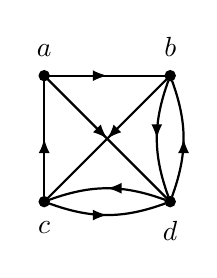
\begin{tikzpicture}
  \GraphInit[vstyle=simple]
  \tikzset{VertexStyle/.append style={scale=0.3}}
  \SetGraphUnit{1.6}
  \Vertex{a}
  \EA(a){b}
  \SO(a){c}
  \SO(b){d}
  
  \extralabel{a}{90}{$a$}
  \extralabel{b}{90}{$b$}
  \extralabel{c}{-90}{$c$}
  \extralabel{d}{-90}{$d$}
  
  \tikzset{EdgeStyle/.style = {->-,>=latex}}
  \Edge(a)(b)
  \Edge(c)(a)
  \Edge(b)(c)
  \Edge(a)(d)
  \tikzset{EdgeStyle/.style = {->-,>=latex,bend right=20}}
  \Edge(c)(d)
  \Edge(d)(c)
  \Edge(b)(d)
  \Edge(d)(b)
\end{tikzpicture}
\hspace*{0.2in}
&
\hspace*{0.2in}
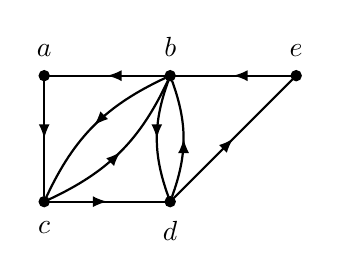
\begin{tikzpicture}
  \GraphInit[vstyle=simple]
  \tikzset{VertexStyle/.append style={scale=0.3}}
  \SetGraphUnit{1.6}
  \Vertex{a}
  \EA(a){b}
  \SO(a){c}
  \SO(b){d}
  \EA(b){e}
  
  \extralabel{a}{90}{$a$}
  \extralabel{b}{90}{$b$}
  \extralabel{c}{-90}{$c$}
  \extralabel{d}{-90}{$d$}
  \extralabel{e}{90}{$e$}
  
  \tikzset{EdgeStyle/.style = {->-,>=latex}}
  \Edge(a)(c)
  \Edge(b)(a)
  \Edge(e)(b)
  \Edge(d)(e)
  \Edge(c)(d)
  \tikzset{EdgeStyle/.style = {->-,>=latex,bend right=20}}
  \Edge(b)(d)
  \Edge(d)(b)
  \Edge(c)(b)
  \Edge(b)(c)
\end{tikzpicture}\\
& \\
(a) \hspace*{0.2in} & \hspace*{0.2in} (b)
\end{tabular}
\end{center}

\solblank
\end{frame}

\begin{frame}
\extitle{Hamilton Paths}
For each of the following graphs, determine whether a Hamilton circuit exists; if so, describe the circuit.  If there is no Hamilton circuit, see if there is a Hamilton path.
\begin{center}
\begin{tabular}{c c c}
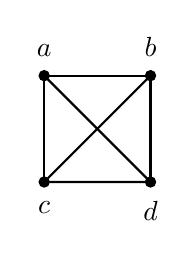
\begin{tikzpicture}[scale=0.45]
  \GraphInit[vstyle=simple]
  \tikzset{VertexStyle/.append style={scale=0.3}}
  \SetGraphUnit{3}
  \Vertex{a}
  \EA(a){b}
  \SO(a){c}
  \EA(c){d}
  
  \extralabel{a}{90}{$a$}
  \extralabel{b}{90}{$b$}
  \extralabel{c}{-90}{$c$}
  \extralabel{d}{-90}{$d$}
  
  \Edge(a)(b)
  \Edge(a)(c)
  \Edge(a)(d)
  \Edge(b)(c)
  \Edge(b)(d)
  \Edge(c)(d)
\end{tikzpicture}
\hspace*{0.15in}
&
\hspace*{0.15in}
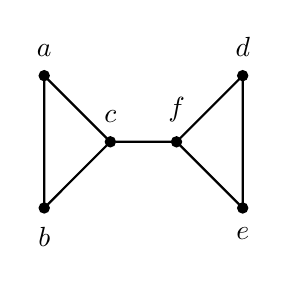
\begin{tikzpicture}[scale=0.35]
  \GraphInit[vstyle=simple]
  \tikzset{VertexStyle/.append style={scale=0.3}}
  \SetGraphUnit{2.4}
  \Vertex{a}
  \SOEA(a){c}
  \SOWE(c){b}
  \EA(c){f}
  \NOEA(f){d}
  \SOEA(f){e}
  
  \extralabel{a}{90}{$a$}
  \extralabel{b}{-90}{$b$}
  \extralabel{c}{90}{$c$}
  \extralabel{d}{90}{$d$}
  \extralabel{e}{-90}{$e$}
  \extralabel{f}{90}{$f$}
  
  \Edge(a)(b)
  \Edge(a)(c)
  \Edge(b)(c)
  \Edge(c)(f)
  \Edge(f)(d)
  \Edge(e)(f)
  \Edge(e)(d)
\end{tikzpicture}
\hspace*{0.15in}
&
\hspace*{0.15in}
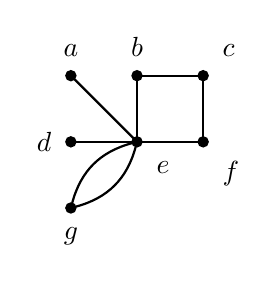
\begin{tikzpicture}[scale=0.35]
  \GraphInit[vstyle=simple]
  \tikzset{VertexStyle/.append style={scale=0.3}}
  \SetGraphUnit{2.4}
  \Vertex{ent}
  \EA(ent){fam}
  \NOEA(ent){liv}
  \NO(ent){kit}
  \NOWE(ent){pan}
  \WE(ent){lau}
  \SOWE(ent){bat}
  
  \extralabel{ent}{-45}{$e$}
  \extralabel{fam}{-45}{$f$}
  \extralabel{liv}{45}{$c$}
  \extralabel{kit}{90}{$b$}
  \extralabel{pan}{90}{$a$}
  \extralabel{lau}{180}{$d$}
  \extralabel{bat}{-90}{$g$}
  
  \Edge(ent)(fam)
  \Edge(ent)(kit)
  \Edge(ent)(pan)
  \Edge(ent)(lau)
  \Edge(fam)(liv)
  \Edge(liv)(kit)
  
  \SetUpEdge[style={bend right=30}]
  \Edge(ent)(bat)
  \Edge(bat)(ent)
\end{tikzpicture}\\
(a) 
\hspace*{0.15in}
&
\hspace*{0.15in}
(b)
\hspace*{0.15in}
&
\hspace*{0.15in}
(c)
\end{tabular}
\end{center}

\solblank
\end{frame}

% Section 8.3
\begin{frame}
\extitle{Nearest Neighbor Algorithm}
Use the nearest neighbor algorithm to find a possible minimum circuit through the Maryland cities shown below, starting and ending at Frederick.
\begin{center}
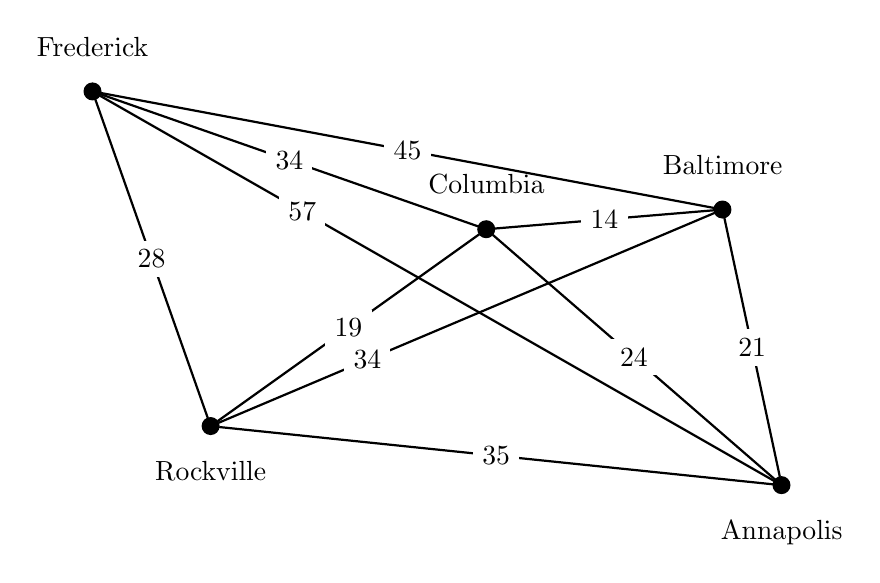
\begin{tikzpicture}[scale=2.5]
  \GraphInit[vstyle=simple]
  \tikzset{VertexStyle/.append style={scale=0.5}}
  \Vertex[x=0,y=0]{Frederick}
  \Vertex[x=3.2,y=-0.6]{Baltimore}
  \Vertex[x=3.5,y=-2]{Annapolis}
  \Vertex[x=2,y=-0.7]{Columbia}
  \Vertex[x=0.6,y=-1.7]{Rockville}
  
  \extralabel[2mm]{Frederick}{90}{Frederick}
  \extralabel[2mm]{Baltimore}{90}{Baltimore}
  \extralabel[2mm]{Annapolis}{-90}{Annapolis}
  \extralabel[2mm]{Columbia}{90}{Columbia}
  \extralabel[2mm]{Rockville}{-90}{Rockville}
  
  \Edge[label=$45$](Frederick)(Baltimore)
  \Edge[label=$34$](Frederick)(Columbia)
  \Edge[label=$28$](Frederick)(Rockville)
  \Edge[label=$14$](Baltimore)(Columbia)
  \Edge[label=$21$](Baltimore)(Annapolis)
  \Edge[label=$19$](Columbia)(Rockville)
  \Edge[label=$24$](Columbia)(Annapolis)
  \Edge[label=$35$](Rockville)(Annapolis)
  \tikzstyle{LabelStyle}=[fill=white,pos=0.3]
  \Edge[label=$34$](Rockville)(Baltimore)
  \Edge[label=$57$](Frederick)(Annapolis)
\end{tikzpicture}
\end{center}
\end{frame}

\begin{frame}
\extitle{Dijkstra's Algorithm}
Use Dijkstra's algorithm to find the shortest path between $a$ and $c$ in the graph shown below.
\begin{center}
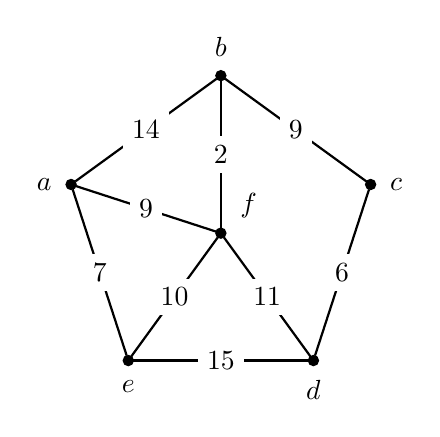
\begin{tikzpicture}
  \GraphInit[vstyle=simple]
  \tikzset{VertexStyle/.append style={scale=0.3}}
  \grEmptyCycle[prefix=a,RA=2,rotation=18]{5}
  \grEmptyCycle[prefix=b,RA=0]{1}
  
  \extralabel{a2}{180}{$a$}
  \extralabel{a1}{90}{$b$}
  \extralabel{a0}{0}{$c$}
  \extralabel{a4}{-90}{$d$}
  \extralabel{a3}{-90}{$e$}
  \extralabel{b0}{30}{$f$}
  
  \Edge[label=14](a2)(a1)
  \Edge[label=7](a2)(a3)
  \Edge[label=9](a2)(b0)
  \Edge[label=9](a1)(a0)
  \Edge[label=2](a1)(b0)
  \Edge[label=6](a0)(a4)
  \Edge[label=15](a4)(a3)
  \Edge[label=11](a4)(b0)
  \Edge[label=10](a3)(b0)
\end{tikzpicture}
\end{center}
\end{frame}

% Section 8.4
\begin{frame}
\extitle{Identifying Trees}
Which of the following are trees?
\begin{center}
\begin{tabular}{c c c}
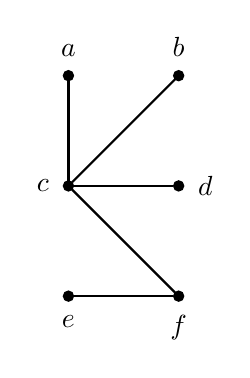
\begin{tikzpicture}
  \GraphInit[vstyle=simple]
  \tikzset{VertexStyle/.append style={scale=0.3}}
  \SetGraphUnit{1.4}
  
  \Vertex{a}
  \EA(a){b}
  \SO(a){c}
  \SOEA(a){d}
  \SO(c){e}
  \EA(e){f}

  \extralabel{a}{90}{$a$}
  \extralabel{b}{90}{$b$}
  \extralabel{c}{180}{$c$}
  \extralabel{d}{0}{$d$}
  \extralabel{e}{-90}{$e$}
  \extralabel{f}{-90}{$f$}
  
  \Edge(a)(c)
  \Edge(b)(c)
  \Edge(d)(c)
  \Edge(f)(c)
  \Edge(e)(f)
\end{tikzpicture}
\hspace*{0.2in}
&
\hspace*{0.2in}
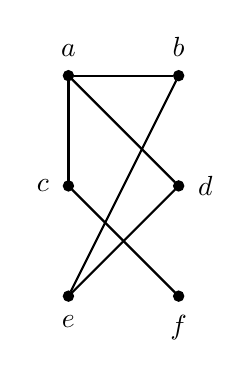
\begin{tikzpicture}
  \GraphInit[vstyle=simple]
  \tikzset{VertexStyle/.append style={scale=0.3}}
  \SetGraphUnit{1.4}
  
  \Vertex{a}
  \EA(a){b}
  \SO(a){c}
  \SOEA(a){d}
  \SO(c){e}
  \EA(e){f}

  \extralabel{a}{90}{$a$}
  \extralabel{b}{90}{$b$}
  \extralabel{c}{180}{$c$}
  \extralabel{d}{0}{$d$}
  \extralabel{e}{-90}{$e$}
  \extralabel{f}{-90}{$f$}
  
  \Edge(a)(c)
  \Edge(a)(b)
  \Edge(a)(d)
  \Edge(b)(e)
  \Edge(c)(f)
  \Edge(d)(e)
\end{tikzpicture}
\hspace*{0.2in}
&
\hspace*{0.2in}
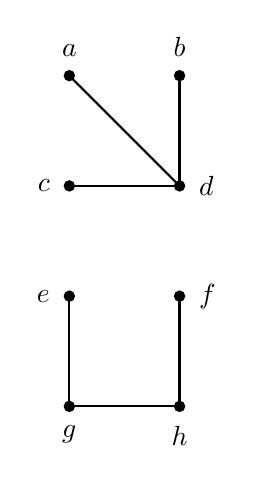
\begin{tikzpicture}
  \GraphInit[vstyle=simple]
  \tikzset{VertexStyle/.append style={scale=0.3}}
  \SetGraphUnit{1.4}
  
  \Vertex{a}
  \EA(a){b}
  \SO(a){c}
  \SOEA(a){d}
  \SO(c){e}
  \EA(e){f}
  \SO(e){g}
  \EA(g){h}

  \extralabel{a}{90}{$a$}
  \extralabel{b}{90}{$b$}
  \extralabel{c}{180}{$c$}
  \extralabel{d}{0}{$d$}
  \extralabel{e}{180}{$e$}
  \extralabel{f}{0}{$f$}
  \extralabel{g}{-90}{$g$}
  \extralabel{h}{-90}{$h$}
  
  \Edge(a)(d)
  \Edge(b)(d)
  \Edge(d)(c)
  \Edge(e)(g)
  \Edge(g)(h)
  \Edge(h)(f)
\end{tikzpicture}\\
& & \\
(a)
\hspace*{0.2in}
&
\hspace*{0.2in}
(b)
\hspace*{0.2in}
&
\hspace*{0.2in}
(c)
\end{tabular}
\end{center}
\end{frame}

\begin{frame}
\extitle{Building a Binary Search Tree}
Build a binary search tree for the following list of words, starting with the first word at the top of the tree:
\begin{center}
\emph{location, solution, promotion, decision, city, bread,\\ enthusiasm, writer, signature, criticism}
\end{center}

\solblank
\end{frame}

\begin{frame}
\extitle{Searching with a Binary Search Tree}
Using the binary tree shown below, search for the word \emph{criticism}.  How many steps (comparisons) are needed to find it?
\begin{center}
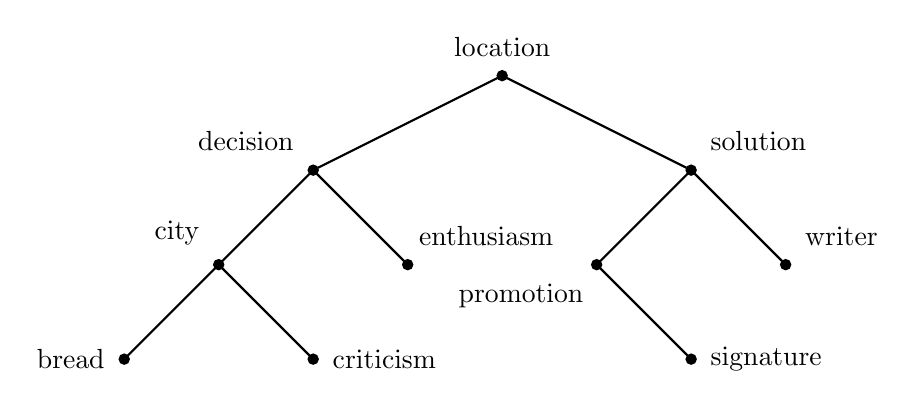
\begin{tikzpicture}[scale=0.6]
  \GraphInit[vstyle=simple]
  \tikzset{VertexStyle/.append style={scale=0.3}}
  
  \Vertex[x=0,y=0]{location}
  \Vertex[x=-4,y=-2]{decision}
  \Vertex[x=4,y=-2]{solution}
  \Vertex[x=-6,y=-4]{city}
  \Vertex[x=-2,y=-4]{enthusiasm}
  \Vertex[x=2,y=-4]{promotion}
  \Vertex[x=6,y=-4]{writer}
  \Vertex[x=-4,y=-6]{criticism}
  \Vertex[x=4,y=-6]{signature}
  \Vertex[x=-8,y=-6]{bread}
  
  \extralabel{location}{90}{location}
  \extralabel{decision}{135}{decision}
  \extralabel{solution}{45}{solution}
  \extralabel{city}{135}{city}
  \extralabel{enthusiasm}{80}{enthusiasm}
  \extralabel{promotion}{250}{promotion}
  \extralabel{writer}{45}{writer}
  \extralabel{criticism}{0}{criticism}
  \extralabel{signature}{0}{signature}
  \extralabel{bread}{180}{bread}
  
  \Edge(location)(decision)
  \Edge(location)(solution)
  \Edge(decision)(city)
  \Edge(decision)(enthusiasm)
  \Edge(solution)(promotion)
  \Edge(solution)(writer)
  \Edge(promotion)(signature)
  \Edge(city)(bread)
  \Edge(city)(criticism)
\end{tikzpicture}
\end{center}
\end{frame}

\begin{frame}
\extitle{Finding a Minimal Spanning Tree}
The graph below shows a network of roads between towns in Nevada.  The roads shown on the graph are unpaved, and the weights represent the length of each road.  Which roads should be paved so that there is a path of paved roads between every pair of towns, and the total length of paved road is as short as possible?  In other words, find a minimal spanning tree for this graph.
\begin{center}
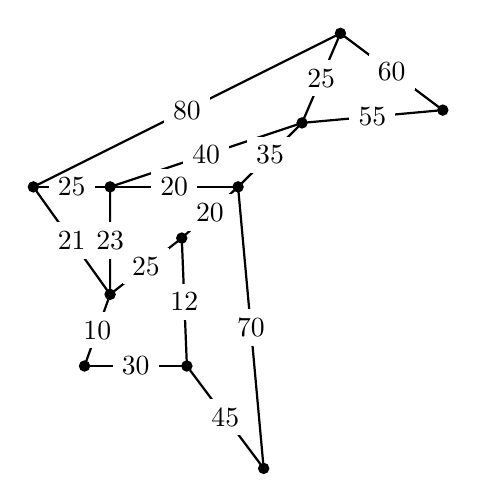
\begin{tikzpicture}[scale=0.65]
  \GraphInit[vstyle=simple]
  \tikzset{VertexStyle/.append style={scale=0.3}}
  
  \Vertex[x=0,y=0]{deepsprings}
  \Vertex[x=2,y=0]{goldpoint}
  \Vertex[x=3.5,y=-2]{beatty}
  \Vertex[x=0.5,y=1.4]{oasis}
  \Vertex[x=1.9,y=2.5]{lida}
  \Vertex[x=-1,y=3.5]{dyer}
  \Vertex[x=0.5,y=3.5]{silverpea}
  \Vertex[x=3,y=3.5]{goldfield}
  \Vertex[x=4.25,y=4.75]{tonopah}
  \Vertex[x=5,y=6.5]{manhattan}
  \Vertex[x=7,y=5]{warmsprings}
  
  %\extralabel{deepsprings}{-90}{Deep Springs}
  %\extralabel[2mm]{goldpoint}{-90}{\parbox{0.5in}{Gold\\ Point}}
  %\extralabel{beatty}{-90}{Beatty}
  %\extralabel{oasis}{180}{Oasis}
  %\extralabel{lida}{0}{Lida}
  %\extralabel{dyer}{180}{Dyer}
  %\extralabel[1mm]{silverpea}{-45}{\parbox{0.5in}{Silver\\ Pea}}
  %\extralabel{goldfield}{0}{Goldfield}
  %\extralabel{tonopah}{-45}{Tonopah}
  %\extralabel{manhattan}{90}{Manhattan}
  %\extralabel{warmsprings}{0}{Warm Springs}
  
  \Edge[label=30](deepsprings)(goldpoint)
  \Edge[label=10](deepsprings)(oasis)
  \Edge[label=12](goldpoint)(lida)
  \Edge[label=45](goldpoint)(beatty)
  \Edge[label=21](oasis)(dyer)
  \Edge[label=23](oasis)(silverpea)
  \Edge[label=25](oasis)(lida)
  \Edge[label=20](lida)(goldfield)
  \Edge[label=70](beatty)(goldfield)
  \Edge[label=25](dyer)(silverpea)
  \Edge[label=80](dyer)(manhattan)
  \Edge[label=40](silverpea)(tonopah)
  \Edge[label=20](silverpea)(goldfield)
  \Edge[label=35](goldfield)(tonopah)
  \Edge[label=25](tonopah)(manhattan)
  \Edge[label=55](tonopah)(warmsprings)
  \Edge[label=60](manhattan)(warmsprings)
\end{tikzpicture}
\end{center}
\end{frame}

\begin{frame}
\extitle{Finding a Minimal Spanning Tree}
Minimal spanning tree:
\begin{center}
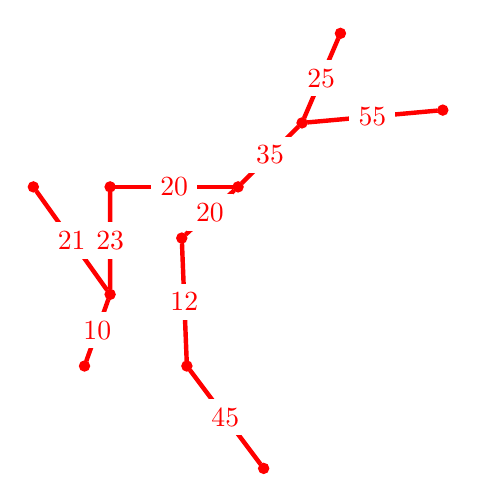
\begin{tikzpicture}[scale=0.65]
  \GraphInit[vstyle=simple]
  \tikzset{VertexStyle/.append style={scale=0.3}}
  
  \tikzset{VertexStyle/.append style={color=red}}
  \Vertex[x=0,y=0]{deepsprings}
  \Vertex[x=2,y=0]{goldpoint}
  \Vertex[x=3.5,y=-2]{beatty}
  \Vertex[x=0.5,y=1.4]{oasis}
  \Vertex[x=1.9,y=2.5]{lida}
  \Vertex[x=-1,y=3.5]{dyer}
  \Vertex[x=0.5,y=3.5]{silverpea}
  \Vertex[x=3,y=3.5]{goldfield}
  \Vertex[x=4.25,y=4.75]{tonopah}
  \Vertex[x=5,y=6.5]{manhattan}
  \Vertex[x=7,y=5]{warmsprings}
  
  %\extralabel{deepsprings}{-90}{\color{red}Deep Springs}
  %\extralabel[2mm]{goldpoint}{-90}{\parbox{0.5in}{\color{red}Gold\\ Point}}
  %\extralabel{beatty}{-90}{\color{red}Beatty}
  %\extralabel{oasis}{180}{\color{red}Oasis}
  %\extralabel{lida}{0}{\color{red}Lida}
  %\extralabel{dyer}{180}{\color{red}Dyer}
  %\extralabel[1mm]{silverpea}{-45}{\parbox{0.5in}{\color{red}Silver\\ Pea}}
  %\extralabel{goldfield}{0}{\color{red}Goldfield}
  %\extralabel{tonopah}{-45}{\color{red}Tonopah}
  %\extralabel{manhattan}{90}{\color{red}Manhattan}
  %\extralabel{warmsprings}{0}{\color{red}Warm Springs}
  
  \SetUpEdge[style={color=red,ultra thick}]
  \tikzstyle{LabelStyle}=[color=red,fill=white]
  \Edge[label=10](deepsprings)(oasis)
  \Edge[label=12](goldpoint)(lida)
  \Edge[label=20](silverpea)(goldfield)
  \Edge[label=20](lida)(goldfield)
  \Edge[label=21](oasis)(dyer)
  \Edge[label=23](oasis)(silverpea)
  \Edge[label=25](tonopah)(manhattan)
  \Edge[label=35](goldfield)(tonopah)
  \Edge[label=45](goldpoint)(beatty)
  \Edge[label=55](tonopah)(warmsprings)
\end{tikzpicture}
\end{center}
\end{frame}
\end{document}